We can give some screen shoots and describes the work here..

For the implementation, we need to consider the correctness of our methods.
\subsection{Detect Directly-follows Graph}


\subsection{Add Long-term Dependency}
This article is used to explain the difficulty I confront about proving the soundness of generated models.
In the first phrase of algorithm, the existing model, positive event log and negative event log are used to generate a new directly-follows graph. Based on Inductiver Miner, this graph is transformed into a sound petri net without long-term dependency. 

In the next phase, our algorithm focuses on detecting and adding long-term dependency in Petri net. We define, if the supported connection on the set pair of xor branches is over a threshold, pair has significant correlation.Therefore, this pair has long-term dependency.

During the implementation, it comes clear that supported connection only on the positive and negative event log is not enough, since the existing model can keep some directly-follows relations about xor branches which do not show in the positive event log or shows only in negative event log. Consequently, when we detect this long-term dependency on those xor branches, there is no evidence of long-term dependency on those xor branches. It results in an unsound model, since those xor branches can't get fired to consume the tokens generated from the choices before.
%% insert one unsound model here and point out the situations. 
\iffalse
\begin{figure}[!h]
	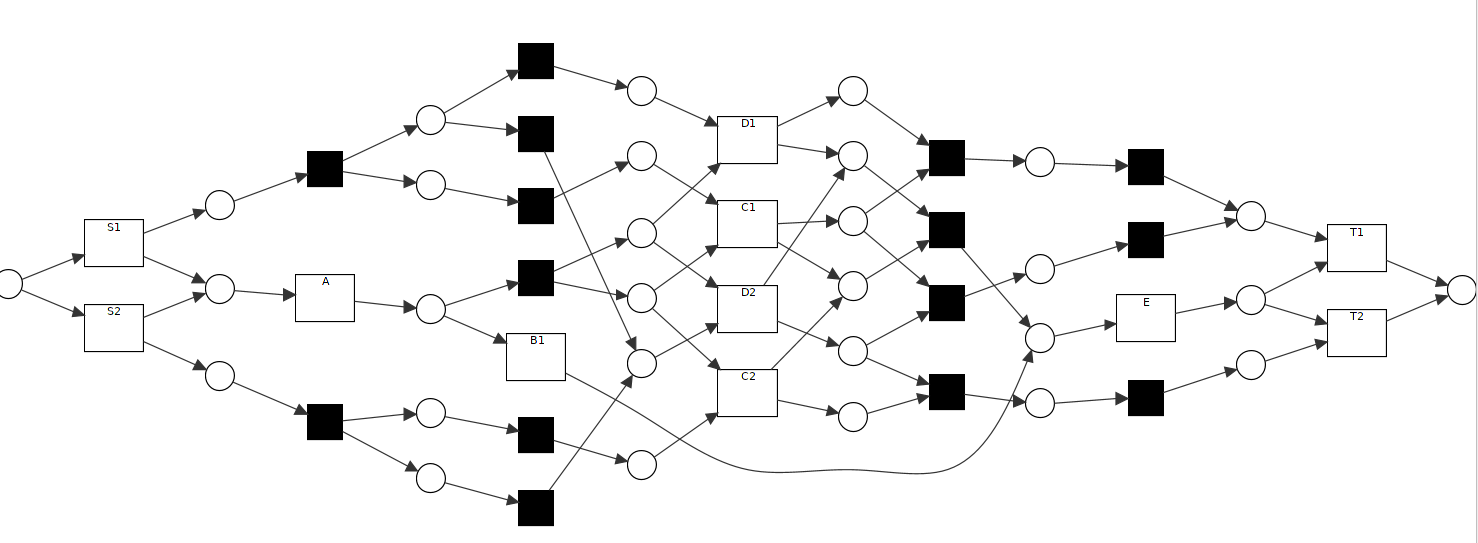
\includegraphics[width=\textwidth]{PN_tc_and_03_01.png}
	\caption{Unsound Repaired Model at Transition B1.}
	\label{fig:unsound_example}
\end{figure}
\fi
\section{Problem Description}
In this section, we use one simple example to deepen our understanding of this problem. 
Given one sound model shown in Fig \ref{fig:seq-2-xor-model} ready for adding long-term dependency on it. 
\begin{figure}[!h]
	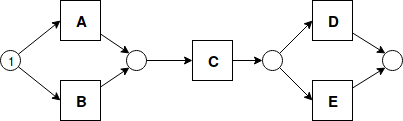
\includegraphics[width=\textwidth]{figures/implementation/LT_Seq_01_Original.png}
	\caption{Simpe Example}
	\label{fig:seq-2-xor-model}
\end{figure}

There are 7 sorts of long-term dependency that is able to happen in this model as listed in the following. Before this, we need to define some concepts at the sake of convenience.
\begin{definition}[Source and Target of Long-term Dependency]
	We define the source set of long-term dependency is  $LT_S:= \{X \vert \exists X, X\rightsquigarrow Y  \in LT \} $, and target set is $LT_T:= \{Y \vert \exists Y, X\rightsquigarrow Y \in LT \} $. \\
	For one xor branch $X \in XORB_S$, the target xor branch set relative to it with long-term dependency is defined as:
	$ LT_T(X)= \{Y \vert \exists Y, X\rightsquigarrow Y \in LT \}$
	Respectively, the source xor branch relative to one xor branch in target is
	$ LT_S(Y)= \{X \vert \exists X, X\rightsquigarrow Y \in LT \}$
\end{definition}
At the same time, we use $XORB_S $ and $XORB_T$ to represent the set of xor branches for source and target xor block. 
\begin{enumerate}
	\item $LT=\{ A\rightsquigarrow D, A\rightsquigarrow E, B\rightsquigarrow D, B\rightsquigarrow D\}$. \\
	$LT_S = \{A,B\}, LT_T=\{D,E\}, \vert LT \vert = \vert XORB_S \vert * \vert XORB_T \vert  $, which means long-term dependency has all combinations of source and target xor branches. 
	\item $LT=\{ A\rightsquigarrow D, A\rightsquigarrow E, B\rightsquigarrow E\}. $\\
	$LT_S = \{A,B\}, LT_T=\{D,E\}$
	$LT_S = XORB_S $ and $LT_T = XORB_T, \vert LT \vert < \vert XORB_S \vert * \vert XORB_T \vert $. it doesn't cover all combinations. But for one xor branch $X \in XORB_S, LT_T(X)= XORB_T$, it has all the full long-term dependency with $XORB_T$. 
	\item $LT=\{ A\rightsquigarrow D, B\rightsquigarrow E\}. $\\
	$LT_S = \{A,B\}, LT_T=\{D,E\}$
	$LT_S = XORB_S $ and $LT_T = XORB_T, \vert LT \vert < \vert XORB_S \vert * \vert XORB_T \vert $. For all xor branch $X \in XORB_S, LT_T(X) \subsetneq XORB_T$, none of xor branch X has long-term dependency with $XORB_T$.
	\item $LT=\{ A\rightsquigarrow D, B\rightsquigarrow D\}.$ \\
	$LT_S = XORB_S ,  LT_T \subsetneq XORB_T$. There exists at least one xor branch $Y \in XORB_T$ which has no long-term dependency on it.
	\item $LT=\{ A\rightsquigarrow D, A\rightsquigarrow E\}.$ \\
	$LT_S \subsetneq XORB_S ,  LT_T = XORB_T$.
	There exists at least one xor branch in source $X \in XORB_S$ which has no long-term dependency on it.
	\item $LT=\{ A\rightsquigarrow E\}. $\\
	$LT_S \subsetneq XORB_S ,  LT_T \subsetneq XORB_T$.
	There exists at least one xor branch in source $X \in XORB_S$  and one xor target xor branch which has no long-term dependency on it.
	\item $ \emptyset$ . There is no long-term dependency on this set. 
\end{enumerate}
For situation 1, it's full connected and xor branches can be chosen freely. So there is no need to add explicit connection on model to represent long-term dependency, therefore the model keeps the same as original. 
For Situation 2 and 3, if $LT_S = XORB_S, LT_T= XORB_T$, then we can create an sound model by adding silent transitions. If not, then we need to use the duplicated transitions to create sound model. But before, we need to prove its soundness. 
For situation 4, 5 and 6, there is no way to prove the soundness even by adding duplicated events. 
For situation 7, I don't think it exists... but if the negative instances has strong effect on it, and make all the connection disappear in long-term dependency but xor branches kept after dfg method??? 
To prove the model sound, we need to prove the four conditions.
\begin{itemize}
	\item safeness. Places cannot hold multiple tokens at the same time
	\item proper completion. If the sink place is marked, all other places are empty.
	\item option to complete. It is always possible to reach the final marking just for the sink place/
	\item no dead part. For any transition there is a path from source to sink place through it. 
\end{itemize}

\section{Discussion of Multiple Implementations}
Until now, multiple methods have been tried to add long-term dependency while trying to keep model sound. Next, we introduce those methods, and give proof if it change its soundness by adding long-term dependency for two xor block in Petri net. 
\subsection{Only Silent Transitions without Duplicated Events}
We add long-term dependency on model by injecting silent transitions and extra places into Petri net. An example is given to describe this method.
\begin{figure}[!h]
	\centering
	\begin{subfigure}[a]{\textwidth}
		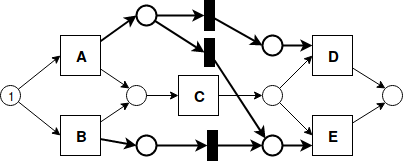
\includegraphics[width=\textwidth]{figures/implementation/LT_Seq_01_Silent_01.png}
		\label{fig:seq-2-silent-1}
		\caption{For situation 2}
	\end{subfigure}
	\hfill
	\begin{subfigure}[b]{\textwidth}
		\centering
		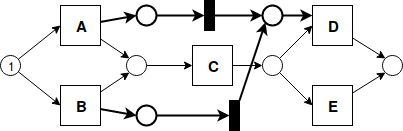
\includegraphics[width=\linewidth]{figures/implementation/LT_Seq_01_Silent_03.png}
		\label{fig:seq-2-silent-2}
		\caption{For situation 4}
	\end{subfigure}
	\hfill
	\begin{subfigure}[c]{\textwidth}
		\centering
		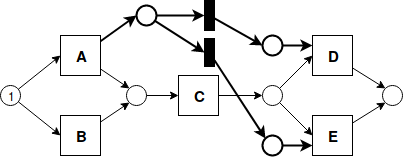
\includegraphics[width=\linewidth]{figures/implementation/LT_Seq_01_Silent_02.png}
		\label{fig:seq-2-silent-3}
		\caption{For situation 5}
	\end{subfigure}
	\label{fig:seq-2-silent-cases}
	\caption{Silent Events for Long-term Dependency}
\end{figure}
This method can not ensure the soundness of model with long-term dependency for situation 4 and 5. \\
\textit{Proof} In Fig \ref{fig:seq-2-silent-2}, it violated the proper completion, and in Fig \ref{fig:seq-2-silent-3}, it can not fire D, E if B is chosen to execute at first. 

\subsection{Full Duplicated Events Without Silent Transitions}
For xor branches which are related to long-term dependency, we duplicate those xor branches in the original xor block, and then connect them together by adding extra place.  An example is given to briefly explain it. 
\begin{figure}[!h]
	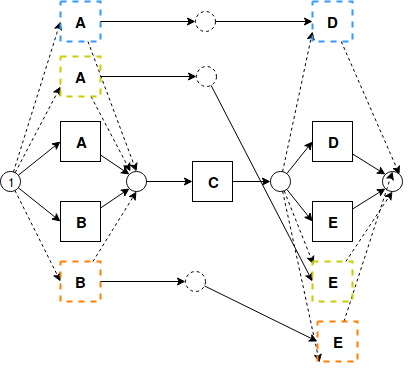
\includegraphics[width=\textwidth]{figures/implementation/LT_Seq_01_FullDuplicated.png}
	\caption{Full Duplicated Events for Long-term Dependency For situation }
	\label{fig:seq-2-full-duplicated}
\end{figure}
In this method, for every item in $LT=\{A\rightsquigarrow D,A\rightsquigarrow E,B\rightsquigarrow D\}$, we duplicate the source and target in corresponding xor block, and then connect the source and target by one explicit place. This method doen not keep the model sound. \\
\textit{Proof:} If original transitions at source xor block are chosen, the execution path is limited to the original transitions in target xor block. It keeps the model sound. If the duplicated transitions at source xor block are chosen (which is colored), two tokens are generated, one for the xor-joint place, one for the extra place. When it comes to target xor block, two kind of transitions are enabled, one is the original transitions, one is the transitions with long-term dependency. But if original transitions are chosen, it violates the proper completion condition for soundness. 

\subsection{Semi Duplicated Events Without Silent Transitions}
This method uses the original transition to express long-term dependency, only adding duplicated events if existing ones are already used for expressing long-term dependency.
\begin{figure}[!h]
	\centering
	\begin{subfigure}[b]{\textwidth}
		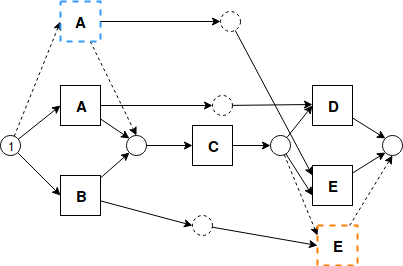
\includegraphics[width=\textwidth]{figures/implementation/LT_Seq_01_SemiDuplicated.png}
		\label{fig:seq-2-semi-duplicated-1}
		\caption{For situation 2}
	\end{subfigure}
	\hfill
	\begin{subfigure}[b]{\textwidth}
		\centering
		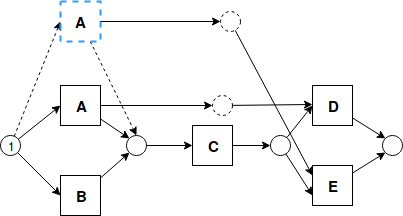
\includegraphics[width=\linewidth]{figures/implementation/LT_Seq_01_SemiDuplicated_Problem2.png}
		\caption{For situation 5}
		\label{fig:seq-2-semi-duplicated-2}
	\end{subfigure}
	\label{fig:seq-2-semi-duplicated-cases}
	\caption{Semi Duplicated Events for Long-term Dependency For situation }
\end{figure}
To express Situation 2 and 3, it create sound model, but for situation 4,5 and 6, it can't guarantee the soundness as shown in the Fig \ref{fig:seq-2-semi-duplicated-2}. Because the transitions in target xor block are not enabled if B is chosen to execute. 

\section{Solution Trials}
To make the generated Petri net sound, there are two thinking ways, one is to make sure that only situation 2 and 3 happen when generating those models. One is to propose a new method to keep it sound. 
In the next subsection, we try to solve this problem by giving constraints to only allow situation 1 2, and 3 available. 
\subsection{Add Constraints}
By adding constraints, we make sure only situations 1,2,3 happen when adding long-term dependency. It requires that after dfg method considers the negative, positive and existing model to delete the unused xor branches for long-term dependency. 
Before doing it, we recover some definitions for long-term dependency detection. 
The definition \ref{def: supported-connection} is rephrased into weight. 
\begin{definition}[Rephrased Correlation of xor branch] The correlation for two branches is expressed into
	\[Wlt(XORB_X,XORB_Y)= Wlt_{ext}(XORB_X, XORB_Y) + Wlt_{pos}(XORB_X, XORB_Y)\] \[ -Wlt_{neg}(XORB_X, XORB_Y)\], where 
	$Wlt_{ext}(XORB_X, XORB_Y)= \frac{1}{|XORB_Y*|}$, $|XORB_{Y*}|$ means the number of possible  directly-follows xor branche set $XORB_{Y*}=\{XORB_{Y1}, XORB_{Y2},...XORB_{Yn} \}$ after $XORB_X$. \\ \\
	$Wlt_{pos}(XORB_X, XORB_Y)= \frac{F_{pos}(XORB_X, XORB_Y)}{F_{pos}(XORB_X, *)}$, \\
	$Wlt_{neg}(XORB_X, XORB_Y)= \frac{F_{neg}(XORB_X, XORB_Y)}{F_{neg}(XORB_X, *)}$, \\	
\end{definition}
The $F_{pos}(XORB_X, XORB_Y)$ and $F_{neg}(XORB_X, XORB_Y)$ are the frequency of the coexistence of $XORB_X$ and $XORB_Y$, respectively in positive and negative event log.

With this rephrased definition, to make the model sound, we need to prove, if there is a xor branch $XORB_Y$ in the generated process tree, there must exist one long-term dependency related to it, $\exists XORB_X, Wlt(XORB_X,XORB_Y) >$ lt-threshold. We formalize this problem. Else, the model can't be sound!!
\begin{proposition}
	Given a process tree, a pair of xor branch set, $(B_A,B_B)$ with $B_A={XORB_{X1}, XORB_{X2},...XORB_{Xm}}, B_B={XORB_{Y1}, XORB_{Y2},...XORB_{Yn}}$, the obligatory part between $B_A$ and $B_B$ is marked M, it is to prove:: \\
	$\forall XORB_Y \in B_B$, if $W(M, XORB_Yj) > threshold$, \\ then there exists one $XORB_Xi \in B_A$ with 
	\[Wlt(XORB_Xi, XORB_Yj)> \text{lt-threshold}\]. 
\end{proposition}
Given a simplified scenes, it is listed in Fig \ref{fig:simplified-graph-model}. M is an obligatory path from the set $\{X1,X2,..Xm\}$ to $\{Y1,Y2,..Yn\}$. If there exists directly-follows relation of M and Y1, then there must exist one long-term dependency of Xi and Y1. 

\begin{figure}[!h]
	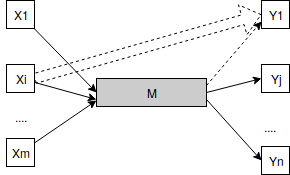
\includegraphics[width=\textwidth]{figures/implementation/RelationOfThreshold-LTThreshold.png}
	\caption{Simplified Graph MOdel}
	\label{fig:simplified-graph-model}
\end{figure}

The definition of $W(M, XORB_{Yj})$ is reviewed below.
\begin{definition}[Assign new weights to graph $G_{new}$]
	there are three weights from $G_{pos}$, $G_{neg}$ and $G_{ext}$, the new weight is 
	\begin{itemize}
		\item For one directly-follows relation, \[ W(E_{G_{new}}(A,B)) = Weight(E_{G_{pos}}(A,B)) + Weight(E_{G_{ext}}(A,B)) - Weight(E_{G_{neg}}(A,B))\]
		\item Given a directly-follows graph G(L), the weight of each directly-follows relation is defined as \[ Weight(E(A,B)) = \frac{Cardinality(E(A,B))}{Cardinality(E(A,*))}  \] 
	\end{itemize}
\end{definition}

When prove by contradiction, we assume that the opposite proposition is true. If it shows that such an assumption leads to a contradiction, then the original proposition is valid. 
\begin{proposition}
	for one xor branch $XORB_Y$, if $W(M, XORB_{Yj}) > threshold$, \\ there exists no one $XORB_{Xi}$ with 
	\[Wlt(XORB_{Xi}, XORB_{Yj})<\text{lt-threshold}\]. 
\end{proposition}

Or we change to another thinking way to get the relation of threshold and lt-threshold, such that we have the theorem valid. Then we rephrase the question into
\begin{proposition}[Another way of thinking]
	Given a process tree, a pair of xor branch set, $(B_A,B_B)$ with $B_A=\{XORB_{X1}, XORB_{X2},...XORB_{Xm}\}, B_B=\{XORB_{Y1}, XORB_{Y2},...XORB_{Yn}\}$, the obligatory part between $B_A$ and $B_B$ is marked M. If,\\
	for one xor branch $XORB_{Yj}$, if $W(M, XORB_{Yj}) > threshold$, \\ there exists one $XORB_Xi$ with 
	\[Wlt(XORB_{Xi}, XORB_{Yj})> \text{lt-threshold}\]
	What is the relation of threshold and lt-threshold?? 
\end{proposition}
If we expand the theorem, we need to prove 
\begin{proposition}[Relation of threshold and lt-threshold]
	What is the relation of threshold and lt-threshold, to make the following proposition valid. If 
	\begin{equation*}
		\begin{gathered}
			W(M, XORB_{Yj})  > threshold \\
			W(M, XORB_{Yj}) = Weight(E_{G_{pos}}(M, XORB_{Yj})) \\
			+ Weight(E_{G_{ext}}(M, XORB_{Yj})) 
			- Weight(E_{G_{neg}}(M, XORB_{Yj})) \\
			\frac{1}{|Y*|} + \frac{\sum_{Xi}{Cardinality(M,Yj|Xi)}} {\sum_{Xi}{Cardinality(M,Y*|Xi)}}  
			- \frac{\sum_{Xi}{Cardinality(M,Yj|Xi)\prime}} {\sum_{Xi}{Cardinality(M,Y*|Xi)\prime} > threshold} \\
			\text{Then, exist one Yj with}\\
			Wlt(Xi, Yj)> \text{lt-threshold} \\
			Wlt{ext}(Xi, Yj) + Wlt{pos}(Xi, Yj) -Wlt{neg}(Xi, Yj) > \text{lt-threshold}\\
			\frac{1}{|Y*|} + \frac{Cardinality(M,Yj|Xi)} {Cardinality(M,Y*|Xi)}  
			- \frac{Cardinality(M,Yj|Xi)\prime} {Cardinality(M,Y*|Xi)\prime} > \text{lt-threshold}  \\
			\text{Or \textbf{there is a contradiction when all Yj}}\\
			Wlt(Xi, Yj)< \text{lt-threshold}\\
			\sum_{Xi} Wlt(Xi, Yj) < |X*|\bullet \text{lt-threshold} \\
			\frac{|X*|}{|Y*|} + \sum_{Xi}\frac{Cardinality(M,Yj|Xi)} {Cardinality(M,Y*|Xi)}  
			- \sum_{Xi}\frac{Cardinality(M,Yj|Xi)\prime} {Cardinality(M,Y*|Xi)\prime} < |X*|\bullet \text{lt-threshold}  \\
		\end{gathered}
	\end{equation*}	
	$Cardinality(M,Yj|Xi)$ means the frequency of coexistence of M and Yj given Xi in the trace in positive, while $Cardinality(M,Yj|Xi)\prime$ represents the frequency in negative. $Cardinality(M,Y*|Xi)$ is the sum frequency of set ${Y1,..Yj,..Yn}$, it equals to \[Cardinality(M,Y*|Xi) = \sum_{Yi}Cardinality(M,Yj|Xi)\]
\end{proposition}
If we set them into zero, there is a lot of existing edges kept into the old method with no evidence in event log to support the connection. 

\subsection{New Method Proposal}
we can add silent transition to make the model sound??? To combine the duplicated events and silent transitions. But how is it and how to prove its soundness?? 

The problem is around situation 4 ,5 and 6. If we have the negative evidence to avoid the long-term dependency. 
For situation 4, $LT=\{ A\rightsquigarrow D, B\rightsquigarrow D\}$. It shows in those two situations. 
\begin{itemize}
	\item If E is kept due to the existing model, and no positive and negative evidence is given for long-term dependency, then Wlt is positive to add long-term dependency on it. 
	\item If long-term dependency is prohibited due to the negative instances, so we need to delete the execution of E by substituting it by silent transitions, and then deleted from the model. Further, after deleting those events, we check the long-term dependency again. If it have full long-term dependency combination, no need to explicitly address them in the model. Else, the explicit long-term dependency is kept in the model. 
\end{itemize}
We can solve it by adding silent transitions in the xor blocks to represent the long-tem dependency. 
\begin{figure}[!h]
	\centering
	\begin{subfigure}[b]{\textwidth}
		\centering
		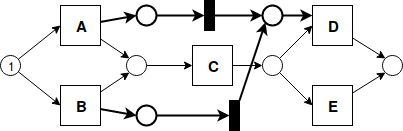
\includegraphics[width=\linewidth]{figures/implementation/LT_Seq_01_Silent_03.png}
		\label{fig:seq-2-silent-2-original}
		\caption{For situation 4}
	\end{subfigure}
	\hfill
	\begin{subfigure}[b]{\textwidth}
		\centering
		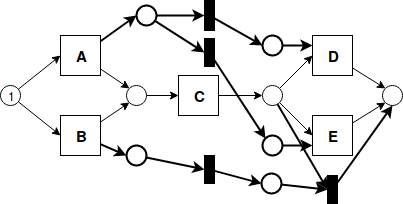
\includegraphics[width=\linewidth]{figures/implementation/LT_Seq_01_Silent_03_AfterAddition.png}
		\label{fig:seq-2-silent-afteraddition}
		\caption{For situation 4}
	\end{subfigure}
	\hfill
	\begin{subfigure}[c]{\textwidth}
		\centering
		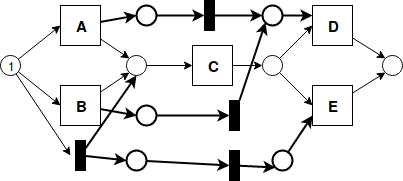
\includegraphics[width=\linewidth]{figures/implementation/LT_Seq_01_Silent_02_AfterAddition.png}
		\label{fig:seq-2-silent-afteraddition-2}
		\caption{For situation 5}
	\end{subfigure}
	\label{fig:seq-2-silent-changes}
	\caption{Silent Events for Long-term Dependency}
\end{figure}

\iffalse
In this way, the final generated models with respect to Fig \ref{fig:seq-2-silent-2} and \ref{fig:seq-2-silent-3} are changed to sound model. 
\begin{figure}[!h]
	\centering
	\begin{subfigure}[b]{\textwidth}
		\centering
		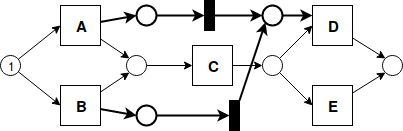
\includegraphics[width=\linewidth]{figures/implementation/LT_Seq_01_Silent_03.png}
		\label{fig:seq-2-silent-2-original}
		\caption{For situation 4}
	\end{subfigure}
	\hfill
	\begin{subfigure}[b]{\textwidth}
		\centering
		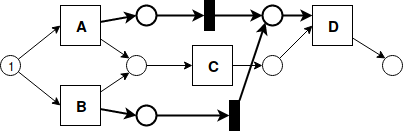
\includegraphics[width=\linewidth]{figures/implementation/LT_Seq_01_Silent_03_AfterDeletion.png}
		\label{fig:seq-2-silent-afterdeletion}
		\caption{For situation 4}
	\end{subfigure}
	\hfill
	\begin{subfigure}[c]{\textwidth}
		\centering
		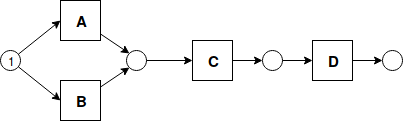
\includegraphics[width=\linewidth]{figures/implementation/LT_Seq_01_Silent_03_AfterDeletion_02.png}
		\label{fig:seq-2-silent-afterdeletion-2}
		\caption{For situation 5}
	\end{subfigure}
	\label{fig:seq-2-silent-changes}
	\caption{Silent Events for Long-term Dependency}
\end{figure}
The similar procedure is done in situation 5, the event B is deleted from the original model, which results in Fig \ref{fig:seq-2-silent-5}.  For situation 6, we combine the procedure for situation 4 and 5, and get the model in Fig \ref{fig:seq-2-silent-6}.
\begin{figure}
	\centering
	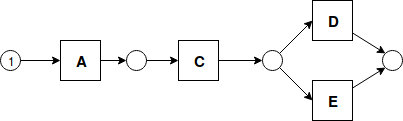
\includegraphics{images/LT_Seq_01_Silent_02_AfterDeletion.png}
	\caption{Caption}
	\label{fig:seq-2-silent-5}
\end{figure}
\begin{figure}
	\centering
	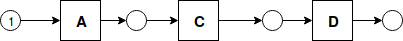
\includegraphics{figures/implementation/LT_Seq_01_Silent_04_AfterDeletion.png}
	\caption{Caption}
	\label{fig:seq-2-silent-6}
\end{figure}
We need to prove the cutting makes the model sound!! By deleting the unused events in target xor block, token passes through another exclusive xor branches. 
Is there any cases that it affects another xor block?? The answer is Yes, if those block is used as source xor block, and it leads to positive long-term dependency, then we need to keep it here!! Deletion causes trouble, too!!  
\fi

More details here are around 6 pages